Chapter \ref{ch:approach} has formalized the problem and put forward a novel framework for finding useful words, consisting of two major functionalities:
Vocabulary list generation, and vocabulary list evaluation.
The list evaluation approach, described in chapter \ref{sec:experimental-setup-with-ai}), utilizes the performance of an AI model, corpus, proxy task as a proxy metric for language ability, in order to estimate how efficiently the vocabulary list may help a human language learner acquire competency.

The list generation approach, proposed in chapter \ref{sec:list-generation}, additionally uses Explainable AI as a tool for analyzing the interaction of the AI model with the corpus to compile vocabulary lists that approach maximal efficiency.

In this chapter, we will describe our implementation, mostly of the list generation approach.
This is because the list evaluation method will be used in chapter \ref{ch:evaluation} as one among several metrics for evaluating the efficiency of vocabulary lists generated by the implementation in this chapter.
However, the evaluation with our approach will use the same components as the list generation approach, such as the chosen corpora, AI models, and NLP tasks.

The first chapter described the implementation of the list generation approach from a system design perspective, describing the interaction between the individual components.
The choice of components in the system is then argued in the following chapters, each of which will feature section describing the desiderata of the component choice are and why, followed by the selection of concrete components.
\todo{Write rest of introduction when chapter structure stands. }

\section{Data Pipeline}

This chapter will give a top-level overview of our implementation for the list generation approach described in chapter \ref{ch:evaluation}.

As mentioned before, the main components of this approach are:

\begin{itemize}
	\item An NLP task, which models a language ability of a language learner.
	\item An AI model, used as a test subject.
	\item A context-specific corpus, to model a language context.
	\item An XAI method, which analyzes the interaction of the AI model with the corpus to determine word utilities.
	\item If the XAI method allows: A tokenizer, determining the words to be analyzed.
\end{itemize}

Thus, the implementation of the approach will consist of determining how exactly these components interact, as well as deciding which model, which XAI method, etc., will be used.

The interaction of these components can be seen in pseudocode in Algorithm \ref{alg:efficient-list-generation}.

\begin{algorithm}
\caption{Efficient List Generation.}
\label{alg:efficient-list-generation}
\begin{algorithmic}[1]
\Require corpus, model, xai\_method
\State Initialize $line\_word\_utilities$ with empty list

\For{each $line$ in $corpus$}
    \State $word\_utilities\_for\_this\_line \gets$ xai\_method$(model, line)$
    \State Append $word\_utilities\_for\_this\_line$ to $line\_word\_utilities$
\EndFor

\State $corpus\_word\_utilities \gets$ aggregate($line\_word\_utilities$)
% \State $corpus\_word\_utilities\_scores$ $\gets$\newline
% aggregate\_word\_utilities($line\_word\_utilities\_scores$)

\State $voc\_list \gets$ words ordered by $corpus\_word\_utilities$

\State \Return $voc\_list$
\end{algorithmic}
\end{algorithm}


The choice of individual components will be tackled by the following chapters.
Because of some dependencies between the components, not all of these components have their own chapter:
The NLP task performed depends on the AI model that we use, as most AI models are trained on only one task.
Therefore, the choice of AI model is discussed together with the NLP task in the next chapter.


\section{NLP Tasks and AI Models}
The NLP task and the corpus used for list generation

There are many NLP tasks we could choose from \tocite{huggingface NLP task list or something}.
But not all are equally suitable.
This chapter will first put forward criteria for selecting NLP tasks in chapter \ref{sec:nlp-tasks-desiderata} for word utility evaluation.
Afterwards, we use these criteria to select a few NLP tasks as appropriate in chapter \ref{sec:nlp-tasks-selection}.
The NLP tasks we choose will dictate the format of our input data, i.e., the corpora we can use.
Therefore, the selection of corpora will be discussed in the next chapter.

\subsection{Desiderata} \label{sec:nlp-tasks-desiderata}

\contentdescription{
	{
			\begin{itemize}
				\item Support many languages
				\item Be as close to human need as possible
				\item $\rightarrow$ task should show general language understanding
				\item data is easy to acquire
				\item $\rightarrow$ data should be freely available for lots of contexts
				\item $\rightarrow$ no need for manual labeling data
			\end{itemize}
		}}

This section will put forward four criteria for selecting NLP tasks for word utility extraction:
The availability of many multilingual AI models and corpora usable as input for the task, generality of the task and ease of evaluation.
These criteria will be used in the next chapter to select concrete tasks for our implementation.

\subsubsection{Model Availability in Many Languages}
The goal of this work is to find approaches to find useful words for the purpose of language learning.
Much research in Natural Language Processing is dedicated to improving NLP performance in English and other high-resource languages such as Spanish, French or Mandarin Chinese \tocite{resource availability in various languages}.
This has the consequence that many AI models and other NLP methods achieve high levels of performance only in these languages, and many AI models are only available in English or a only small number of languages.
However, there are over 7,000 languages in the world \tocite{Ethnologue}, and for many of these there exist corpora, or online digital texts which could hypothetically be used as inputs for our word utility extraction approach.
For this reason, our implementation strives to realize word utility extraction in \textbf{as many languages as possible}.

\subsubsection{Corpus Availability in Many Languages}
The second point of consideration for task selection is \textbf{how much data is available for performing the task}.
Ideally, we would like tasks for which suitable corpora are freely available or can be trivially generated from available corpora.
This is for the reason that, with a larger amount of usable data, we not only improve the accuracy of our approach, but also increase the diversity of input data.
With diverse input data available, we have a larger amount of linguistic contexts for we can find utilities, and the context-specific language learning is a central motivation of this work.

\subsubsection{Generality of Skill Required}
Another important point to consider when selecting an NLP task is \textbf{how general the linguistic skills} are that the task requires:
We use the performance in the NLP task as a proxy metric for the test subject's language ability.
As such, we must ensure that task reflects a general level of semantic understanding, not only a narrow mechanistic skill that can be accomplished by using only a small part of the input.

\subsubsection{Ease of Evaluation}
To ensure we can measure the performance, we must also choose a task whose results can be easily compared with each other:
Some tasks, such as text summarization, present a challenge for automatic evaluation:
It is difficult to put a number on how similar two summaries of a text are.
While evaluation measures, such as BLUE scores\tocite{BLEU}, exist, it is questionable how well they capture the similarity between texts, because they do not recognize the semantic similarity of synonyms, and a different sentence structure will result in a low BLEU score even if the actual meaning of the sentences may be very close.
It follows that if we have the freedom to choose NLP tasks whose results can be automatically evaluated with a fair degree of accuracy, we should choose them.


\subsubsection{Summary}
To summarize our desiderata for NLP tasks:
Our implementation seeks to use NLP tasks for which both AI models and corpora exist in a large number of languages, to maximize accuracy and diversity of linguistic contexts which can be modeled.
We prefer tasks that demonstrate general language understanding over tasks that only require a narrow skill set to perform or that are too technical, because general tasks are expected to align more with human linguistic skills.
Finally, the task must be easily scorable, since the task score is the metric by which we gauge how useful words are.

The next section will present several tasks which fulfill the above criteria, and explain what consequences their selection has on the other components of vocabulary list generation.
The choice of NLP tasks employed to test a XAI-based approach for word utility estimation is a crucial step:
Since we are trying to estimate the utility a word a word has to language understanding, the NLP tasks should reflect language understanding as much as possible.

\subsection{Task Selection} \label{sec:nlp-tasks-selection}
A good place to start looking for such tasks are those which are typically employed for pre-training NLP models:
Pre-training tasks are used to first endow the AI model with a general understanding of the language, before using transfer learning to specialize it for a more specific downstream task.
Such tasks must necessarily be general and require general language understanding, since training the model with them is supposed to provide a solid basis for a wide variety of NLP tasks.
Another benefit of using pre-training tasks is that their training is unsupervised, meaning there is no need to manually label data.
\todo{Look at various pre-training tasks, preferably those used by state-of-the-art AI models}
\todo{include free availability for AI models in their justification}

\subsection{NLP Pre-Training Tasks Used by State-of-the-Art AI Models}
This section takes a look at the pretraining process of recent state-of-the-art LLM models which have made public their training process.
Both the NLP tasks and the kind of data is considered.


\begin{description}
	\item[GPT-4] \cite{openaiGPT4TechnicalReport2024}

	      Task: Language modeling (see next section).

	      Data: Not disclosed in detail, according to the original paper, the model was trained "using both publicly available data (such as internet data) and data licensed from third-party providers".
	\item[GPT-3] \cite{brownLanguageModelsAre2020}
	      GPT-3 is a model that does not rely on transfer learning to apply its linguistic understanding to new tasks; instead, it uses zero-shot and few-shot learning to perform tasks it was not specifically trained for.

	      Task: Language modeling (same as GPT-2 \cite{radfordLanguageModelsAre2019})

	      Data: Common Crawl, WebText2, Books1, Books2, Wikipedia \todo{link sources?}
	\item[LLama 3.3] \cite{LlamamodelsModelsLlama3_3}


	      Task: Meta did not make public the training process for Llama 3.3.

	      Data: "data from publicly available sources"
\end{description}

\subsection{Tasks Considered}
\begin{description}
	\item[Next Sentence Prediction]
	      In this task, the AI model takes as input two sentences and predicts a probability for the second sentence being the successor of the first sentence in their source text.
	      Advantages for this task for our purposes is that such a dataset is easy to generate, as it merely requires a corpus of sentences that follow from each other, which is easily obtained from Wikipedia articles, film subtitles, or any other continuous text.

	\item[Text summarization]
	      This task involves summarizing a given text, in other words, writing a shorter version of the input text while still conveying as much of the information from the original text as possible.
	      Summarizing texts seems to require a high level of "understanding" of the text and would thus seem to be good choice for testing whether ablating certain words from the text would have detrimental effect on the model performance.
	      Unfortunately, this task requires hand-labeled datasets and is thus not a good candidate if we aim to find approaches which can be implemented in many different languages, as there is a dearth in data in many of the less-studied languages of the world.

	\item[Masked language modeling (aka. "cloze task")]
	\item[Causal language modeling (aka. Next token prediction)]
	\item[Sentence order prediction]
	\item[Sentence embeddings]
	      Sentence embeddings take the approach of transforming words into meaningful vectors and extend it to whole sentences.
	      This "task" differs from the others in that we do not measure differences in performance when the input is perturbed; but rather a distance between the embedding vectors themselves.
	      This justification for such an approach is that sentences whose meaning is very different should end up further apart from each other in the vector space once embedded.
	      This brings several advantages:
	      This approach can be performed on any corpus containing distinct sentences.
	      These corpus does not have to be document-level, and sentences need not be consecutive.
	      To make this a task on which XAI methods can be applied, we can define a distance from the original token
\end{description}

\subsection{Sentence Embedding Methods}

\begin{description}
	\item[LASER] \cite{artetxeMassivelyMultilingualSentence2019}
	\item[BERT] \cite{reimersMakingMonolingualSentence2020}
\end{description}

\subsection{Data Required for Each NLP Task}
The various NLP tasks employed require certain types of corpora to be employed properly:

\begin{itemize}
	\item[Next sentence prediction]
	      Requires a corpus that contains consecutive sentences.
	      Furthermore, NSP typically predicts whether two sentences follow each other in a document, not a dialogue (see the data on BERT training \cite{kentonBertPretrainingDeep2019}).
	      This excludes movie subtitles from the possible corpora for this task.

\end{itemize}

\subsection{AI Models}
\begin{itemize}
	\item NSP-model ABC
	\item LLAMA?
\end{itemize}

\todo{tests of performance tests of models used with corpora used (e.g., if NSP prediction model is reliable)}


\section{Corpora}
The previous section has put forth criteria for which NLP tasks should be used in our word utility evaluation approach.
The other core component of the approach is the input data used to perform the experiments, as it serves the purpose of modeling the language contexts in which the language learner is striving to achieve proficiency.
This chapter will therefore first lay out the general selection criteria for corpora.
We will then introduce some publicly available corpora which are suitable for our evaluation approach, as well as propose data augmentation methods to increase their usefulness further.



\subsection{Desiderata}

\contentdescription{
	{
			For the purposes of this paper, it was desirable that the corpora used be:
			\begin{itemize}
				\item representative of what language learners strive for
				\item freely available in many languages
				\item can be split up into diverse linguistic contexts
				\item for NSP: must be comprised of documents for continuous sentences
			\end{itemize}
		}}

This section will put forward our general criteria for corpus selection, following from our overarching goal of using the model to model linguistic contexts for the purpose of language learning.
\todo{when the following subsection stand, summarize here}
\todo{when actual corpora are decided: Mention them in throughout this chapter too}


\subsubsection{Document-Level Corpus}
The first desideratum for our corpora stems from our choice to use Next Sentence Prediction as one of our NLP tasks:
As Next Sentence Prediction predicts whether one sentence is likely the continuation of another, it requires continuous sentences pairs to work.
To generate these pairs, we must use (at least some) corpora featuring continuous tests, not only individual sentences.
This presents a challenge, as many corpora which are compiled from Web Crawls, such as the Common Crawl dataset \footnote{\url{https://commoncrawl.org/}}, present independent single lines, mostly because single sentences cannot be put under copyright in many states \tocite{copyright being the reason for non-document level corpora}
One solution to this would be make a dataset from crawling various news pages ourselves.
However, Wikipedia contains articles one many different topic which do not underlie strict copyright license (see the section on Wikipedia), thus for this work, we opted not to compile our own document-level corpus.

\subsubsection{Free Availability in Many Languages}
In chapter \ref{sec:nlp-tasks-desiderata} we put forward reasons for why freely available AI models which can handle a diverse pool of languages are desirable for our undertaking.
By the same token, we also prefer corpora which are publicly available in many languages over corpora which only include data in one language.
While a monolingual corpus is not inferior to a multilingual one, its use necessitates that the user manually compile many corpora if a multilingual implementation is to be achieved.

\subsubsection{Closeness to Linguistic Contexts Desired by Language Learners}
As mentioned before, the corpus in our word utility extraction approach serves the purpose of modeling a linguistic context, and this linguistic context should reflect some set of situations that a language learner is likely to find themselves in.
Typical situations would include reading the news, reading literature or watching movies in their target language.
As such, corpora which are close to the materials which language learners are likely to engage with are desirable, since their use makes the AI model's performance on the task more reflective of skills that a language learner would like to acquire.

\subsubsection{Diversity of Linguistic Contexts within Corpus}
Not only the relevance of the entire corpus's linguistic context is important:
Some corpora enable us to further split them up into smaller corpora with more specific language contexts.
For instance, while we can use a corpus such as \textit{Wikipedia} as a whole, the structure of Wikipedia enables us to group articles by the category they belong to (politics/sports etc.), as well as split them by subheading (History/Introduction/etc.) to find more specific contexts.
Such corpora are especially efficient for generating multiple contexts, hence we will make use of such corpora.



\subsection{Corpora Used}
\subsubsection{OpenSubtitles Parallel Corpus}
This set of corpora contains parallel corpora:
Corpora which has text segments in one language aligned with the presumed translation of the segment in a second language.
Its sentences are generated from subtitles from the popular subtitle sharing platform \textit{OpenSubtitles} (https://www.opensubtitles.org/) and undergo various preprocessing and filtering steps as described in \cite{lisonOpensubtitles2016ExtractingLarge2016}.
These include:
\begin{enumerate}
	\item Enforcing universal UTF-8 character encoding.
	\item
	      Splitting and joining of sentences from their original subtitles blocks (the segments which appear on screen when watching the movie with its subtitle).
	      One such block may contain multiple sentences, or only a partial one.
	      There is thus a n-to-m-relationship between the blocks and sentences.
	\item Checking and correcting possible spelling issues, especially ones arising from OCR (Optical character recognition) errors.
	\item From available subtitles, identifying the subtitle pair which is most likely to be accurate in its alignments and free from errors such spelling, taking into account metadata such as user ratings of subtitles.

\end{enumerate}
One advantageous aspect of this corpus is that is contains many sentences that are sequential, which means we can generate a Next Sentence Prediction dataset from it (add hedging here since not all lines in corpus are sequential and even within the same movies there may will be pauses in the subs).
This corpus has been used to train machine translation models such as OPUS-MT \cite{tiedemannOPUSMTbuildingOpenTranslation2020}, a freely available set of transformer models for translation, including between low-resource languages. \todo{Not completely correct, the pipeline uses data from OPUS, not necessarily or specifically from OpenSubs}
While it is possible to reconstruct which movies the subtitle lines came from from information contained in the corpus, it is unfortunately not clear how these movies were selected in the first place.


The full process, as illustrated by the authors, can be seen in figure \ref{fig:opensubs pipeline}
As of 2025, the latest version of the corpus (v2018) contains aligned subtitles of 62 languages between each other.

\begin{figure}[H]
	\centering
	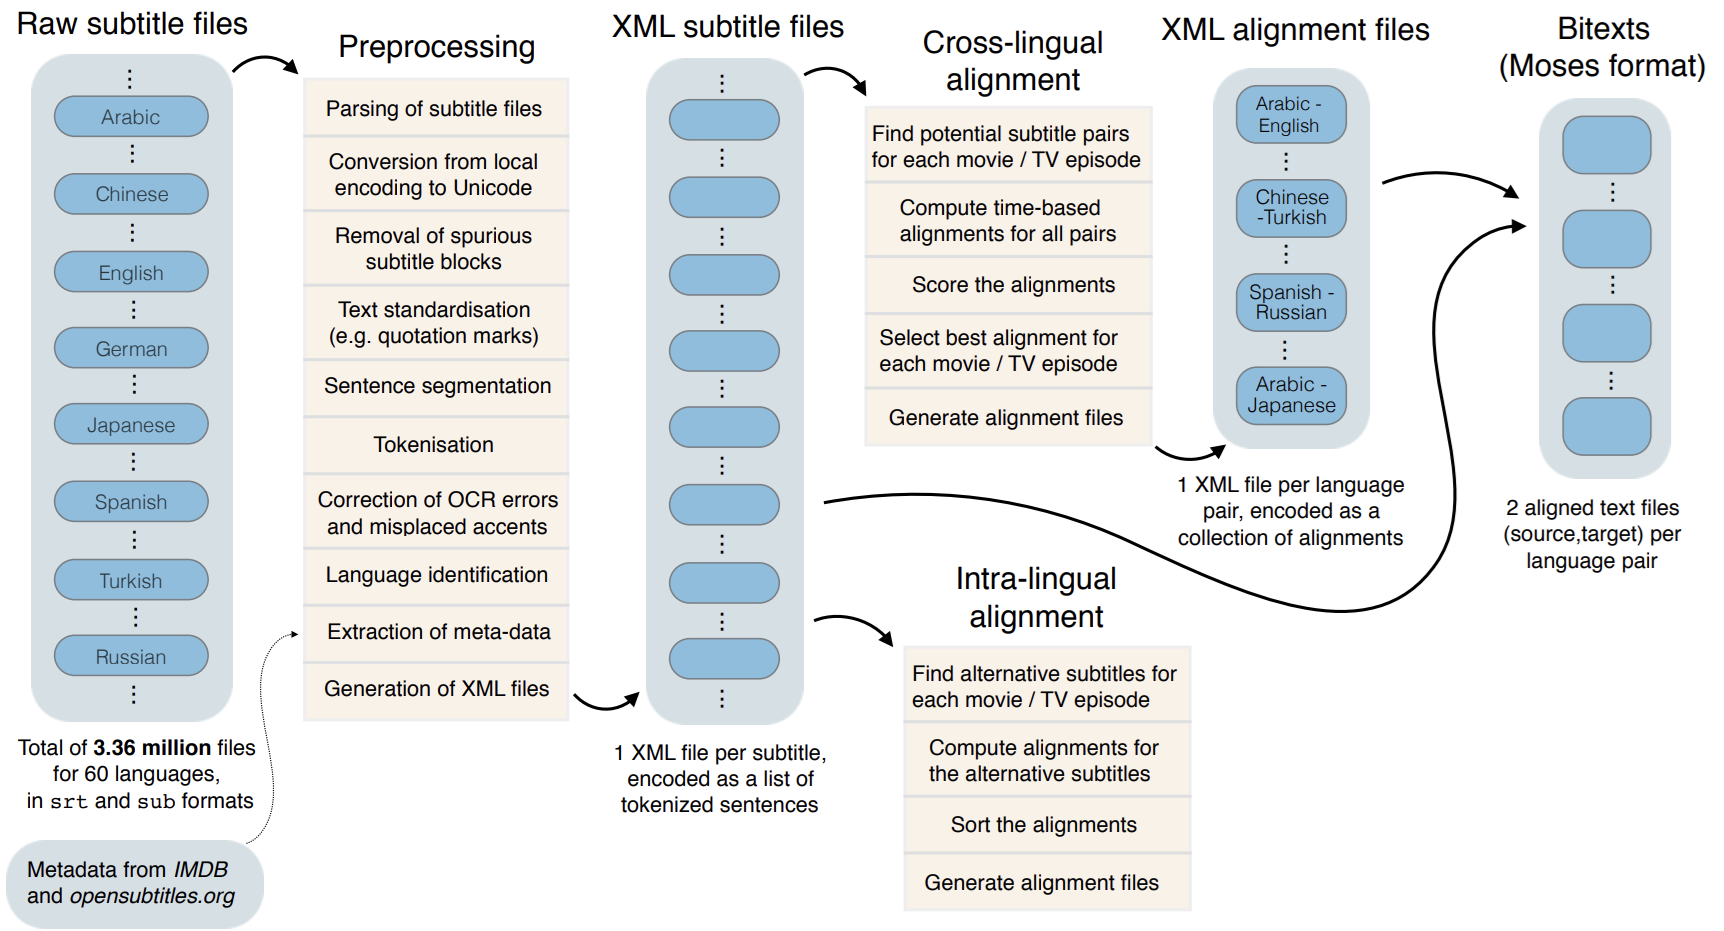
\includegraphics[width=\textwidth]{opensubs_corpus_processing.png}
	\caption{The pipeline producing the OpenSubtitles parallel corpus}
	\label{fig:opensubs pipeline}
\end{figure}

\subsubsection{Wikipedia}
\contentdescription{{
			\begin{itemize}
				\item advantages: diversity of topics, document level corpus which is not copyrighted, regularly updates dumps
				\item disadvantages: language is technical, does not resemble spoken conversation
				\item describe grouping intro multiple scope corpora: describe category structure of Wikipedia
			\end{itemize}
		}}

Wikipedia offers a large amount of data which can be downloaded in the form of dumps at \url{https://dumps.wikimedia.org/}.
In this work, these dumps will be valuable in modeling various linguistic contexts that a language learner might be interested in.

\paragraph{Advantages:}

Wikipedia is a valuable resource for several reasons:
It contains a vast number of articles, from a diverse set of topics.
Wikipedia articles have category assigned to them, which we can use to group articles into linguistic contexts
This means we do not have to assign the articles to topics ourselves, thus enabling the creation of many smaller-scope corpora from Wikipedia with minimal effort.
The characteristics of the article category system on Wikipedia will be discussed in the paragraph below.

Another upshot of Wikipedia is that its articles are licensed under the Creative Commons Attribution-ShareAlike 4.0 International License (\textit{CC BY-SA}).
Because of this, Wikipedia can provide dumps of its entire article database ready for download, with the articles in continuous form and with category metadata attached to them.
This enables us to use the articles as a source for Next Sentence Prediction NSP task.

\paragraph{Disadvantages:}
While Wikipedia offers a large diversity of articles and article topics, the language of the articles follows an academic style of writing.
Thus, the diversity in registers is comparatively low:
Wikipedia is less likely to contain informal language, such as nonstandard language (English: \textit{ain't}, \textit{y'all}) and slang.

Furthermore, it features little language taking conversational form.
% This means that e.g., for English, the second person pronoun "you" occurs very infrequently on Wikipedia. \tocite{Wikipedia rank of you}
This is especially relevant for languages where the certain grammatical forms signify something about the relationship between the speaker and listener:
In Japanese, there exist various linguistic markers of politeness (\textit{Teineigo} and \textit{Keigo}) which play a crucial role in in-person interactions between Japanese speakers, as their presence or absence can signify respect, familiarity or humility with regards to one's interlocutor.
However, such forms are rarely found on Wikipedia, as it does not take the form of a person addressing another person or persons.
Thus, we can see that texts on Wikipedia are of limited use to model linguistic contexts involving in-person conversion.

With these advantages an disadvantages in mind, this work uses Wikipedia articles and their associated metadata to make corpora of various sizes, as will be seen in the next section.

\paragraph{Modeling Linguistic Contexts}

One of the chief advantages of Wikipedia as a corpus its diversity of covered topics.
A language learner who is interested in a particular topic will likely find a matching article category on Wikipedia:
For example, a person with an interest in American cinema who is learning English could likely take vocabulary from the articles of the category "20th-century American actresses" to boost their language learning in that linguistic context.
For this reason, we use a number of manually selected categories as testing grounds for our list generation approach.
For each category, we use a number of articles to make a list, then use different articles from the same category as testing data in the evaluation.
We can thus check if learning vocabulary from a category genuinely prepares a learner in understanding texts from that context.

At the same time, a learner could also wish to make a vocabulary list from concrete Wikipedia articles they would like to read.
For that reason, also use single articles as corpora to be processed by our list generation approach.
In that case, no split of training and test data is necessary, as the aim is not to model general knowledge about a domain, but equip the learner with vocabulary about the \textbf{closed} context of a Wikipedia article.
Therefore in the single-article approach, both the list generation and evaluation use all lines of the article.


% \paragraph{Wikipedia's Category System for Articles}
% There are x categoris on Wikipedia.
% Each article may belong to one or more categories.
% One category can have 0:n parent categories, 0:n child categories.
% Categories therefore not not follow a tree structure, thus most articles belong to more than one top-level category.



\subsubsection{Leipzig Wortschatz Corpora}
Available in x languages

But: data quality issues, methodology might be outdated

\cite{goldhahnBuildingLargeMonolingual2012}

\subsubsection{CCMatrix / NLLB}

% \subsection{Data Augmentation}
% Data Augmentation was not used to gain additional data.
% While in recent years data augmentation methods have become popular for training AI models in NLP, most of these would have either no or a detrimental effect on the methods employed in this paper:
% Some of these methods include \cite{pellicerDataAugmentationTechniques2023}:
% \begin{description}
% 	\item[Character level]
% 	      Introducing character swaps to data is a method used to train the model to noise in the data, but in our case, would only add noise to the results.
% 	\item[Word level]
% 	      There exist techniques to switch words for synonyms or swap words in the sentences to create noise.
% 	      As with noise on the word level, adding words in inappropriate places is undesired for our use case.
% 	      Swapping words for synonyms would also prove detrimental, as this would skew the statistics away from the natural word distribution found in the human-generated source texts.
% \end{description}
% Higher level techniques suffer from the same issues.
% For this reason, the data is left in its "natural state" for our purposes.
%

\section{XAI Methods} \label{sec:xai-methods}
In order to appraise the influence of words in a corpus on the performance of the AI model performing and NLP task, this work employs Explainable AI methods, as explained in chapter \ref{sec:xai-as-tools-of-analysis}.

\subsection{Desiderata}
Chapter \ref{sec:explainable-ai} has explained the use of XAI and stated what kind of XAI methods are especially appropriate for our purpose:
We will employ local, feature attribution XAI methods of both model-specific and model-agnostic type, as these will allow use to gauge the importance of words in the input from multiple points of view.
Model-specific methods have an advantage in that they typically do not require many model calls to attribute importances to features, and take the model structure into account.
On the other hand, model-agnostic methods are useful in that they can be used on any model and gauge the input-output relationship by performing actual experiments on the model, by observing the way changes to input change the output of the model.

In addition to these taxonomical specifications, an ideal XAI method for word extraction should be both accurate in its feature attributions and should not require extensive computation.
Apart from the benefit of attaining faster results, a computationally lightweight approach allows the model to process more data in less time, presumably boosting the accuracy of the resulting utility evaluation.

In the following sections, we will propose several concrete XAI methods for use with the described list generation approach.
The relationship of the XAI methods to the NLP tasks will also be discussed, as not every XAI method is feasible with every tasks, either because of unrealistic amount of computation or because the results of the combination are difficult to evaluate.
The results of the experiments with these methods will be seen in chapter \ref{ch:evaluation}.
\todo{argue against approaches where the input is reduced to BOW, such as SHAP}

\subsection{Model-Agnostic Approaches}
\contentdescription{
	Single Token Ablation, Progressive Summary with
}

\subsubsection{Single Token Ablation}
Our aim in using XAI methods is to find out which words, if known, improve the model's performance the most, when compared to not knowing the word.
Perhaps the simplest way of testing this is by going through every word in the input to the AI model, and checking the model performance when the word is removed from the input.
Within this work, this approach will be known as \textbf{Single Token Ablation}.

\paragraph{Approach:}
Given an input line or pair of lines:
For each word in the input, create a variation of the input where the word is removed.
Run the model on all inputs and measure how much performance is degraded in each case.
Estimated utility is the difference in performance between not removing and removing the word.

\paragraph{Advantages:}
One advantage of Single Token Ablation is its conceptual simplicity, as it is very easy to implement.
Furthermore, its time complexity is fairly minimal for a feature method, as it requires only one model call for each unique token in the sentence ($\mathcal{O}(n)$).

\paragraph{Disadvantages:}
The main downside of this method is that, in long sentences, leaving out a single token will not change the meaning of the sentence to such an extend that the sentence becomes unintelligible.
Assuming the AI model can process sentences with missing words with similar accuracy as humans, the impact on performance may therefore be minimal or not predictive of actual usefulness.
Furthermore, this method does not take into account the utility of a word in the context of word combinations.

\paragraph{Summary:}
Among model-agnostic methods, Single Token Ablation is a computationally inexpensive whose feature perturbation consists of ablating single words.
We may think of this method as simulating a language learner who already knows all words in a sentence except for one, and as such it may not model word utility in such a way that the resulting list is useful for beginners.

\subsubsection{Progressive Summary}
While Single Token Ablation is easy to implement and cheap to execute, its downside is that the performance differences may not be representative of actual utility.
To achieve a more accurate evaluation, we may think of a approach that is in some sense the inverse of removing single words from sentences:
Checking which words are the most essential by reducing the sentence a minimal number of words.

\paragraph{Approach:}
Given an input line, we first let the AI model run on the unaltered input.
We then go through every word in the input line, let the model run with the single word as input, and check which of the words produces an output that is close to the output for the unaltered line.
We can thus see which word summarized the sentence the best.

However, we need not stop here:
After determining the most essential word in the sentence, we can check which words from the remaining pool of words brings the outputs closer still.
By iterating this method, we progressively reconstruct the original sentence, which each step being the best next word to add in order to restore the original output.
For this reason, we will refer to this method as \textbf{Progressive Summary}.
Here, the estimated utility of a word is the boost in performance which is brought to the sentence when the word is added.

\paragraph{Advantages:}
The Progressive Summary approach models the perception of a beginner-level language learner better than Single Token Ablation.
The latter asks which single word, when lacking, degrades performance the most.
Progressive Summary instead asks which words, if known, bring language performance closest to knowing all words in the sentence.

\paragraph{Disadvantages:}
Progressive Summary is much more computationally intensive than Single Token Ablation, which requires only one model call per word in the sentence.
Because of its iterative approach, for a sentence with 10 words, Progressive Summary calls the model $10+9+8+... $ or $\sum_{i=1}^{n}i = \frac{n^2 + n}{2}$ times, which is a time complexity of $\mathcal{O}(n^2)$.


\paragraph{Compatibility with NLP tasks}
As Progressive Summary starts from a set of one words and then progresses to larger sets, it is difficulty to meaningfully employ in combination with an NLP task whose input is not a single line, e.g., Next Sentence Prediction.
One could circumvent the issue by leaving one of the sentences in its original form and only perturbing the other, but this can hardly be seen as a modeling of natural language ability.

\todo{Maybe: Describe issues of using PS with models whose output is single number: Approximating with single words may not be meaningful approximation at all. But should test empirically.}

As such, our implementation Progressive Summary is not used with Next Sentence Prediction.

\paragraph{Summary:}
Progressive Summary attempts to find the most important words in a sentence one by one, by first reducing the sentence to one word, then two etc., and using a distance metric to compare the "summaries" to the original sentence.
The words which bring the model output for the summary closest to that of the original sentence are regarded as the most useful.

\subsection{Model-Specific Methods}
The model-agnostic methods so far are general tools which can be employed on any model.
However, as many of the latest state-of-the-art AI models follow the Neural Network architecture, and more specifically the transformer architecture (see chapter \ref{sec:transformer}), we will also attempt word utility estimation with methods specific to these model.
These model-specific XAI methods have the advantage of being computationally efficient:
Model-agnostic methods extract information about the model by perturbing its inputs and analyzing the resulting changes in the output.
This requires many model calls for one input datum.
In contrast, model-specific methods can analyze the input-output relationship with only one model call, as they look into the model itself for information.
We will therefore try two model-specific methods for analyzing word utility as well, as their more efficient calculations means they can process more input data in a given time, which should increase the accuracy of the resulting word list.

\subsubsection{Attention as Explanation}
One XAI method which has been proposed to explain the decision of transformer models specifically is the transformer's own attention mechanism:
As stated in chapter \ref{sec:transformer}, transformer model use attention to focus on some inputs over others.
This may be used as a kind of explanation, as the inputs which receive more attention presumably contribute more to the model's decision than those with less attention.

\paragraph{Approach:}
Let a transformer model run on an input line.
The transformer will attribution an attention value to each token in the input.
Normalize the attentions such that the attention for all words in the line sums up to one.
The attributed attention to a word is its estimated utility.

\paragraph{Advantages:}
As hinted at before, this method uses one model call for one input line, and thus has a time complexity of $\mathcal{O}(1)$.


\paragraph{Disadvantages:}
One disadvantage of Attention as our attention mechanism is that attentions are attributed to input tokens of the model.
Unlike the black-box methods where word masking is controlled by a tokenizer \textit{independent of the model}, the tokenizer cannot be changed.
AI models are trained with some tokenizer as preprocessing the input, and this tokenizer cannot be changed, lest we change the input format to the AI model itself.
This is an issue because it means that lists generated with the model-specific tokenizer are not necessarily comparable to lists from model-agnostic methods, as the tokenization method may differ.
Additionally, many tokenizer which are used in the preprocessing of models tokenize on a \textit{sub-word} level:

In addition to this technical downside, Attention is controversial as a mechanism to explain model decisions.
\tocite{Attention is not Explanation}

\paragraph{Summary:}


\subsubsection{Layer-wise Relevance Propagation (not yet implemented $\rightarrow$ may be deleted)}
\paragraph{Approach:}
\paragraph{Advantages:}
\paragraph{Disadvantages:}
\paragraph{Summary:}


